\documentclass[12pt, letterpaper]{report}
\usepackage[a4paper, margin=0.7in, top=20mm, bottom=20mm]{geometry}
\usepackage{mathspec}
\usepackage[UTF8]{ctex}
\usepackage[colorlinks=true, linkcolor=black, urlcolor=blue]{hyperref}
\usepackage{listings}
\usepackage{xcolor}
\usepackage{graphicx}

\graphicspath{ {C:/Programming/MIT6.828_OS/pics/} }

% ---- Code Section Style ----
\colorlet{mygray}{black!30}
\colorlet{mygreen}{green!60!blue}
\colorlet{mymauve}{red!60!blue}

\lstdefinelanguage
   [x64]{Assembler}     % add a "x64" dialect of Assembler
   [x86masm]{Assembler} % based on the "x86masm" dialect
   % with these extra keywords:
   {morekeywords={CDQE,CQO,CMPSQ,CMPXCHG16B,JRCXZ,LODSQ,MOVSXD, %
                  POPFQ,PUSHFQ,SCASQ,STOSQ,IRETQ,RDTSCP,SWAPGS, %
                  rax,rdx,rcx,rbx,rsi,rdi,rsp,rbp, %
                  r8,r8d,r8w,r8b,r9,r9d,r9w,r9b, %
                  r10,r10d,r10w,r10b,r11,r11d,r11w,r11b, %
                  r12,r12d,r12w,r12b,r13,r13d,r13w,r13b, %
                  r14,r14d,r14w,r14b,r15,r15d,r15w,r15b}} % etc.


\lstset{
  backgroundcolor=\color{gray!10},  
  basicstyle=\ttfamily,
  columns=fullflexible,
  breakatwhitespace=false,      
  breaklines=true,                
  captionpos=b,                    
  commentstyle=\color{mygreen}, 
  extendedchars=true,              
  frame=single,                   
  keepspaces=true,             
  keywordstyle=\color{blue},                    
  numbers=none,                
  numbersep=5pt,                   
  numberstyle=\tiny\color{blue}, 
  rulecolor=\color{mygray},        
  showspaces=false,               
  showtabs=false,                 
  stepnumber=5,                  
  stringstyle=\color{mymauve},    
  tabsize=3,                      
  title=\lstname                
}

\lstdefinestyle{CStyle}{  
    % commentstyle=\color{mGreen},
    % keywordstyle=\color{magenta},
    % numberstyle=\tiny\color{mGray},
    % stringstyle=\color{mPurple},
    basicstyle=\footnotesize,
    breakatwhitespace=false,                              
    showstringspaces=false,
    language=C
}

\lstdefinestyle{AssemblyStyle}{  
    basicstyle=\footnotesize,
    breakatwhitespace=false,                              
    showstringspaces=false,
    language=[x64] Assembler
}


\lstdefinestyle{MakeFileStyle}{  
    basicstyle=\footnotesize,
    breakatwhitespace=false,                              
    showstringspaces=false,
    language=[gnu] make
}


% ----------------------------


\setcounter{chapter}{0}
\setlength{\parindent}{2em}
\setmainfont{Times New Roman}
\setcounter{tocdepth}{1}
\setcounter{secnumdepth}{1}

\title{MIT6.828 Lab1: Booting a PC}
\author{Zhuofan Zhang}
\date{December 2021}



\begin{document}
\maketitle
% ---- Contents ----
\pagenumbering{roman}
\renewcommand\contentsname{\Huge Contents}
\tableofcontents{}
% ------------------


% ---- Part A ----
\newpage
\pagenumbering{arabic}
\chapter[\Large PC Bootstrap]{PC Bootstrap}
\section[\large Getting Started with x86 assembly]{Getting Started with x86 assembly}
本节内容主要为熟悉基本的x86汇编语言,此处归纳总结一些基本的语法内容。
\lstset{style=AssemblyStyle}
\setmainfont{Consolas}
\begin{lstlisting}
##### Three kinds of OPERANDs #####
# %xxx -- Register
# $num -- Immediate(eg: $0x1F, $-577)
# (%xxx) -- memory access

##### Addressing Mode #####
# Immediate Addressing
# Register Addressing -- eg: MOV AX, BX (means "copy data in AX to BX")
# Direct Addressing(memeory written in instruction) -- eg: MOV AX, [2000H]
# Indirect Addressing -- eg: MOV AX, [BX]
# Indexed Addressing
# Offsetting Addressing

##### Directives #####
# .global {symbol1,symbol2,...} 
# -- declares each symbol in the list to be global(can be seen by the linker).
# .set {symbol} {expression} -- assigns the value of expression to symbol.
# .data -- The .data directive changes the current section to .data.
# .codexx 
# -- instructs the assembler to interpret subsequent instructions as exact bits.(eg: .code16, .code32)
\end{lstlisting}
\setmainfont{Times New Roman}

除了基本的语法规则外,需注意x86为分段内存管理(Segment):
寄存器 CS/DS/EX 分别为代码段、数据段及额外段寄存器,当指令中未指定段地址时默认使用这三个寄存器
内的值。具体情况根据CPU运行于实模式(Real Mode)或保护模式(Protect Mode)而不同,将在后文详述。 \par

\subsection{\large Exercise 1}
\textsl{ Familiarize yourself with the assembly language materials.
         You don't have to read them now, but you'll almost certainly 
         want to refer to some of this material
         when reading and writing x86 assembly.} \par
\quad \par
本节内容是对x86体系及其汇编的熟悉练习。6.828 Ref 中提供了x86的手册,其中比较重要的查阅内容为
 \textsl{Volume 3A: System Programming Guide PART I} 一册,该册对IA32的架构有简单的介绍,并对
硬件与软件之间的约定有明确的描述。\par 
\quad \par
{
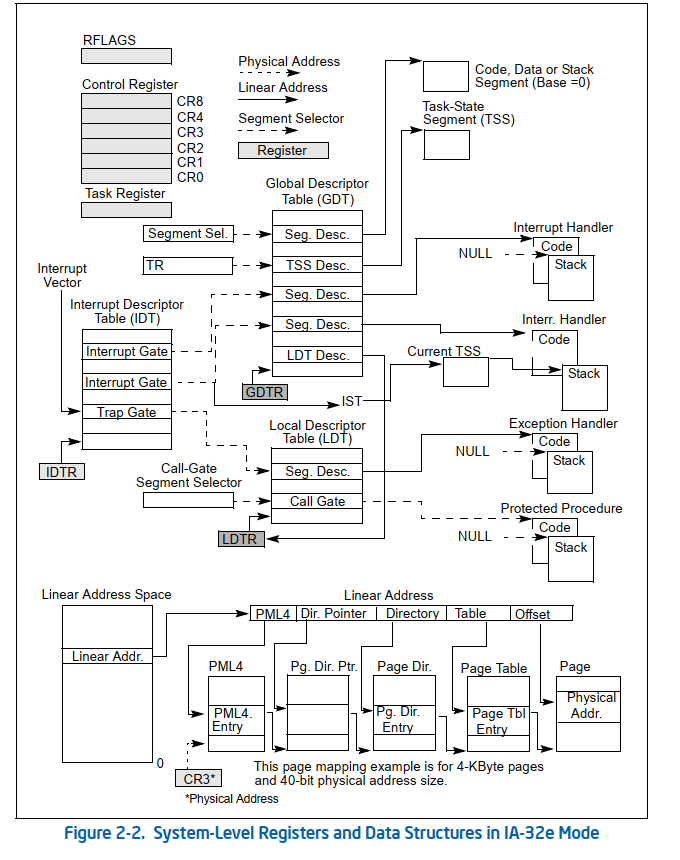
\includegraphics[width=\textwidth,height=0.78\textheight]{IA32-syslevel}
}
\quad \par
\section[\large Simulating the x86]{Simulating the x86}
本节主要内容是介绍课程实验中工具的基本使用方法。实验使用QEMU仿真器对x86硬件进行模拟,
并借助GDB进行调试。

\section[\large The PC's Physical Address Space]{The PC's Physical Address Space}
在启动PC前,首先了解一些关于\textsl{物理地址空间(Physic Address Space)}的内容。x86-CPU系列有一个相对固定的
物理地址空间,如下图所示。\par

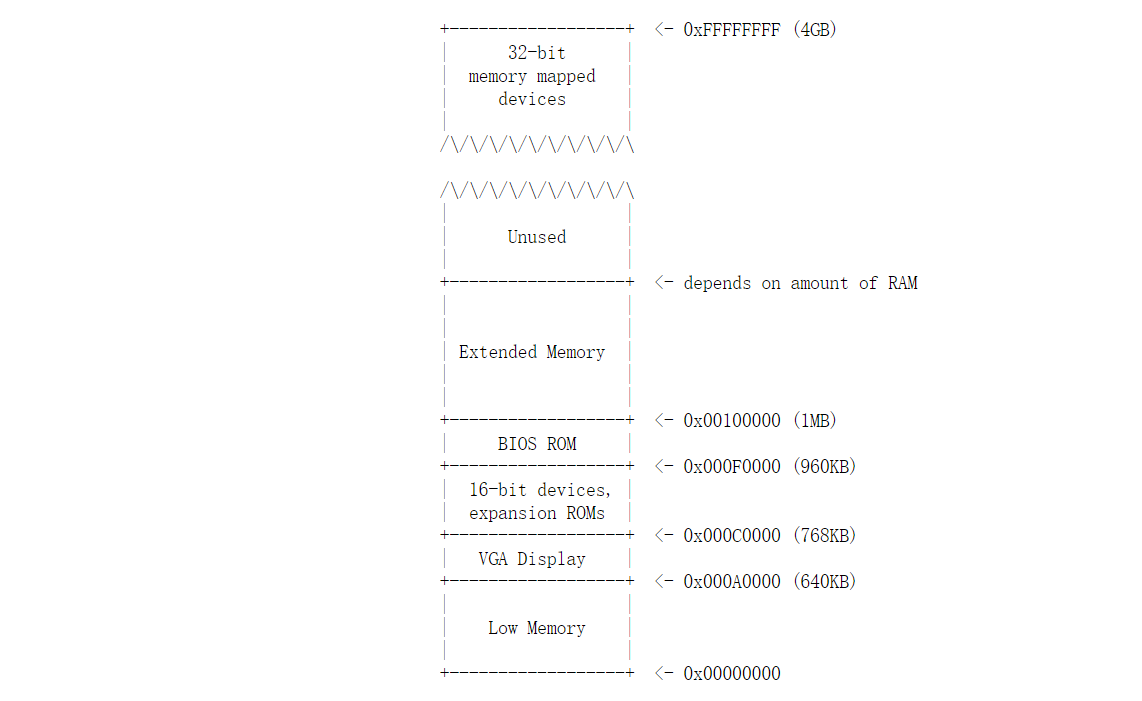
\includegraphics[width=\textwidth]{PC_PhysicalAddressSpace}
早期的8088处理器只使用1MB内存,对应于此物理空间的低位1MB,除去固定提供给BIOS和VGA等使用的地址,
余下的Low Memory即为早期处理器实际可用的内存空间。其后的处理器为保证前向兼容而保留这一模式,增加
Extend Memory。此外,BIOS在整个地址空间的最高处保留一小段空间,提供给32-bit的PCI设备使用。\par
当前处理器扩展至64-bit后,为保证前向兼容,32-bit物理空间的模式依然得到保留(也即,为PCI设备保留的
这段地址依然存在)。\textbf{本实验构建的JOS操作系统只使用256MB的物理内存,因此所有的内容假设建立在32-bit物理空间上}。\par

\section[\large The ROM BIOS]{The ROM BIOS}
PC的启动流程基本可以概括为:1.CPU正常启动;2.读取并运行BIOS;
3.BIOS进行设备初始化,加载BootLoader;4.BootLoader加载内核,并将控制流交给内核。\par 
早期BIOS烧写在ROM中,一旦设置便不可修改。现代PC可以使用其他方案进行初始化,
但统一归类为BIOS程序(或常见写作BIOS Legacy)。BIOS会将主板可以检测到的所有IO设备初始化,
最后将控制交给加载完成的BootLoader。\par
使用GDB进行程序追踪可发现,CPU启动后第一条指令的位置:
\lstset{style=AssemblyStyle}
\setmainfont{Consolas}
\begin{lstlisting}
[f000:fff0]    0xffff0: ljmp   $0xf000,$0xe05b
\end{lstlisting}
\setmainfont{Times New Roman}
可以看到,它正好落在上一节提到的BIOS地址空间中。\par 
不同的BIOS基本功能都包括上电自检(Power On Self Test, POST)及主板设备的初始化。
BIOS系统按照一定顺序从硬盘或USB存储设备/网络上寻找操作系统,并从第一个扇区中找到BootLoader,将控制
交给它,开始对内核的加载。\par 

\subsection{\large Exercise 2}
\textsl{Use GDB's si (Step Instruction) command
         to trace into the ROM BIOS for a few more instructions, 
         and try to guess what it might be doing. } \par 
\quad \par 
这个Exercise是探究BIOS执行的指令及作用。BIOS基本功能我们在本节中已阐述,具体的命令
属于dirty knowledge,此处不展开详细讨论。详细的分析指出此处 BIOS主要进行中断描述表的设置、
初始化设备、\textbf{寻找可以加载的设备并读取其Boot Loader,将控制权交给它}。Boot Loader 相关内容
将在下一节中详述。


\chapter[\Large The Boot Loader]{The Boot Loader}
\section[\large Loading the Kernel I: boot.S]{Loading the Kernel I: boot.S}
BIOS在找到可启动的设备后,会将设备中第一个扇区(512KB)的内容加载到 0x7c00 位置,
并跳转至此处运行。这一个扇区中的代码一般用于将OS加载到内存中,称之为\textsl{加载器(BootLoader)}。
JOS的BootLoader源码由 boot/boot.S 及 boot/main.c 两部分组成。 \par

boot.S 文件中的源码主要完成了以下工作:1.关闭中断;2.段寄存器置0;3.A20地址线使能;
4.从实模式切换到保护模式,加载GDT;5.将控制交给 boot/main.c/bootmain()。 \par

A20线使能同样源于向前兼容性问题。8086/8088处理器仅有20条地址线(实模式下0-FFFF:FFFF地址空间);
而在80286后的x86处理器地址线多于20条,为了向前兼容,在实模式下对A20线置零;当切换到保护模式后,
解除地址空间的限制。\par 

从\textsl{实模式(Real Mode)}切换到\textsl{保护模式(Protect Mode)}是 boot.S 的核心功能。\par 
实模式是早期x86处理器的工作模式。当时的处理器使用20条地址线(1MB的物理地址空间),而寄存器均为16-bit大小。
为实现对整个地址空间的索引,使用了\textbf{段基址:段偏移}的分段策略:计算地址时将段基址左移4位后与偏移量相加,
得到最终的物理地址,其中段基址一般由\textbf{段寄存器}给出。在本次Lab中,切换至实模式前可以看到指令地址显示
诸如 [f000:fff0] 即为这种寻址模式的表示。
由于段基址和段偏移两个信息即可推出实际地址,故称为“实”模式。\par 
\textsl{保护模式(Protect Mode)}是进入32-bit地址空间后,为了提高寻址安全性及灵活性所设计的新策略。为了与之前的
架构体系相兼容,仍使用段寄存器组,但此时其中存放的不再是段基址,而是\textsl{段选择子(Segment Selector)}。
段选择子是使用\textsl{全局描述符表(Global Descriptor Table, GDT)}后产生的概念。GDT中存放的表项也称为段描述符,其
结构如下图所示,每个段描述符描述一个内存段。(JOS中使用 \textbf{struct Segdesc} 描述。)\par
\quad \par
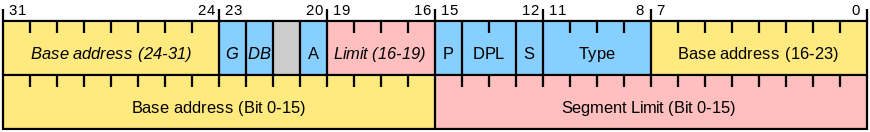
\includegraphics[width=0.8\textwidth]{GDTEntry}
\quad \par
\quad \par
\quad \par
在此基础上,段选择子可看作GDT的索引,其结构如下图所示。\par 
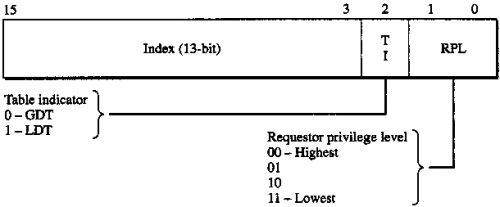
\includegraphics[width=\textwidth]{SegmentSelector}
需要补充的是,除了GDT外,x86架构提供另一个结构:\textsl{本地描述符表(Local Descriptor Table, LDT)}。
LDT与GDT拥有相同的结构和类似的功能,两者的区别在于:GDT主要是为操作系统提供内存索引服务,而LDT则为用户
进程等提供相似的服务。因此,GDT一般在操作系统中作为孤本保存,而LDT通常有多个不同副本,且LDT会被保存在GDT中。\par 
结合上文,我们最终可以得到在x86保护模式下的寻址方式(如下图所示)。\par 
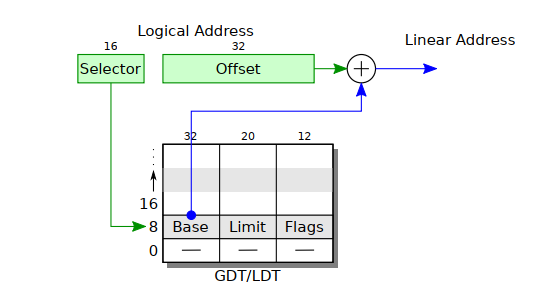
\includegraphics[width=0.8\textwidth]{GDT}


\section[\large Loading the Kernel II: bootmain.c]{Loading the Kernel II: bootmain.c}
{
        在 boot.S 完成准备工作后,控制权交到 boot/main.c/bootmain() 中。
        这部分源码的核心是将内核加载到内存中,并将控制权交给内核,完成启动。在本次实验中,内核以ELF文件形式存在。\par 
        加载内核的核心是 readseg() 和 readsect() 两个函数。根据 main.c 中提供的定义,内核ELF文件将被加载到
        物理地址 0x100000 处。bootmain() 会首先加载ELF Header部分检查文件是否有效并确认文件大小,最后再将整个内核
        加载到物理内存中。
} \par 

\subsection{\large Exercise 3}
\textsl{
        Set a breakpoint at address 0x7c00, 
        which is where the boot sector will be loaded. 
        Continue execution until that breakpoint. 
        Trace through the code in boot/boot.S 
        and compare the original boot loader source code with 
        both the disassembly in obj/boot/boot.asm and GDB.
} \par 

\textsl{
        Trace into bootmain() in boot/main.c, and then into readsect(). 
        Identify the exact assembly instructions that correspond to each of the statements in readsect(). 
        Trace through the rest of readsect() and back out into bootmain(), and identify the begin and end of the for loop 
        that reads the remaining sectors of the kernel from the disk. 
        Find out what code will run when the loop is finished, 
        set a breakpoint there, and continue to that breakpoint. 
        Then step through the remainder of the boot loader.
} \par
\quad \par
\textsl{
        Be able to answer the following questions:
} \par
{
        1. At what point does the processor start executing 32-bit code? 
        What exactly causes the switch from 16- to 32-bit mode?
} \par
{
        2. What is the last instruction of the boot loader executed, 
        and what is the first instruction of the kernel it just loaded?
} \par
{
        3. Where is the first instruction of the kernel?
} \par 
{
        4. How does the boot loader decide how many sectors 
        it must read in order to fetch the entire kernel from disk? 
        Where does it find this information?
} \par 
\quad \par
根据题目的要求我们单步调试并追踪 0x7c00 开始后的代码(即BootLoader),并根据追踪内容回答上述问题:\par 
{
        1. 处理器在 \textbf{ljmp    \$PROT\_MODE\_CSEG, \$protcseg} 处从实模式切换到保护模式,
        证据之一是执行完该指令后GDB的地址显示模式发生了改变;
} \par
\quad \par 
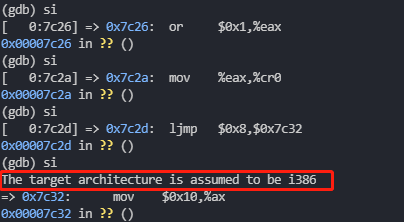
\includegraphics[width=0.8\textwidth]{real2protect}
\quad \par 
{
        2/3. boot loader 执行的最后一条指令是 \textbf{call *0x10018},
        利用 GDB 查看此处内存,正好可以看出其中为地址 0x10000c处的指令,
        故 kernel 第一条指令为该处的: \textbf{movw   \$0x1234,0x472}
} \par
\quad \par  
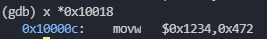
\includegraphics[width=0.8\textwidth]{lastfirst}
\quad \par
{
        4. 可以从 ELF 文件中得知(ELFHDR->e\_phnum)。
} \par 

% 这个Exercise让我们追踪从0x7c00开始的代码(即BootLoader),并比较调试命令与 boot.asm(BootLoader反汇编结果)。
% 通过比较我们可以发现,反汇编文件中给出的命令地址与GDB调试时产生的地址是相同的:这说明,Boot部分的逻辑地址与虚拟地址是相同的。
% 我们可以通过OBJDUMP工具进行验证:
% \lstset{style=AssemblyStyle}
% \setmainfont{Consolas}
% \begin{lstlisting}
% # objdump -h obj/boot/boot.out
% boot.out:     file format elf32-i386

% Sections:
% Idx Name          Size      VMA       LMA       File off  Algn
%   0 .text         0000017e  00007c00  00007c00  00000054  2**2
%                   CONTENTS, ALLOC, LOAD, CODE
%   1 .eh_frame     000000cc  00007d80  00007d80  000001d4  2**2
%                   CONTENTS, ALLOC, LOAD, READONLY, DATA
%   2 .stab         000006d8  00000000  00000000  000002a0  2**2
%                   CONTENTS, READONLY, DEBUGGING
%   3 .stabstr      000007df  00000000  00000000  00000978  2**0
%                   CONTENTS, READONLY, DEBUGGING
%   4 .comment      00000011  00000000  00000000  00001157  2**0
%                   CONTENTS, READONLY
% \end{lstlisting}
% \setmainfont{Times New Roman}
% 这与Kernel部分是不同的:
% \lstset{style=AssemblyStyle}
% \setmainfont{Consolas}
% \begin{lstlisting}
% # objdump -h obj/kern/kernel
% kernel:     file format elf32-i386

% Sections:
% Idx Name          Size      VMA       LMA       File off  Algn
%   0 .text         00004eae  f0100000  00100000  00001000  2**2
%                   CONTENTS, ALLOC, LOAD, READONLY, CODE
%   1 .rodata       00001720  f0104ec0  00104ec0  00005ec0  2**5
%                   CONTENTS, ALLOC, LOAD, READONLY, DATA
%   2 .stab         000089b9  f01065e0  001065e0  000075e0  2**2
%                   CONTENTS, ALLOC, LOAD, READONLY, DATA
%   3 .stabstr      00009d41  f010ef99  0010ef99  0000ff99  2**0
%                   CONTENTS, ALLOC, LOAD, READONLY, DATA
%   4 .data         000c9f51  f0119000  00119000  0001a000  2**12
%                   CONTENTS, ALLOC, LOAD, DATA
%   5 .bss          00000ef4  f01e2f60  001e2f60  000e3f60  2**5
%                   CONTENTS, ALLOC, LOAD, DATA
%   6 .comment      00000011  00000000  00000000  000e4e54  2**0
%                   CONTENTS, READONLY
% \end{lstlisting}
% \setmainfont{Times New Roman}

\subsection{Exercise 4}
\textsl{Read about programming with pointers in C.}\par 
\quad \par
阅读任务,略。

\subsection{Exercise 5}
\textsl{Trace through the first few instructions of the boot loader again 
        and identify the first instruction that would "break" or otherwise 
        do the wrong thing if you were to get the boot loader's link address wrong.
        Then change the link address in boot/Makefrag to something wrong, 
        run make clean, recompile the lab with make, and trace into the boot loader again 
        to see what happens. 
        Don't forget to change the link address back and make clean again afterward!} \par 
\quad \par 
% 修改MakeFlag文件中BootLoader的链接地址(0x7c00),再追踪出现bug的指令。由于BIOS对BootLoader加载的位置
% 是硬编码的,因此实际上BootLoader仍加载到了0x7c00处,并跳转到此处进行。因此理论上,BIOS可以顺利地将控制转交给
% BootLoader。问题出现在链接地址的改变对BootLoader链接时重定向的改变:当链接器根据修改后的链接地址重定向后,
% 如源码中的 lgdt 和 ljmp 命令的操作数都将出现问题。lgdt 命令处出现问题,但JOS依然成功加载了GDT,最后是在 ljmp 指令处
% 发生了错误。
根据Lab的提示,我们修改 boot/Makefrag 中的 -Ttext 选项:从 0x7c00 改为 0x1000。再次使用 GDB 进行单步调试,
可以发现 BootLoader 被正常加载,并在初始化的部分均可以正常执行,直到运行至前面提到的实模式切换到保护模式的
 ljmp 语句时出现问题:无法跳转。 \par
尝试从原理上分析这一问题的原因:由于 BIOS 对可启动设备的加载地址是硬编码的(作为硬件与软件的约定),因此实际上
 BootLoader 依然被加载到了正确的位置,控制权被正确移交;由于实际上一直到加载 LGDT 的指令前所有的代码均不涉及
寻址,因此 BootLoader 此时仍能正常执行;当执行到加载 LGDT 的指令时,实际上已经加载了错误的内容,但仍未发生错误;
直到需要 ljmp 时读取了 LGDT 中加载的错误内容,才发生了错误(无法跳转)。\par 
\quad \par 
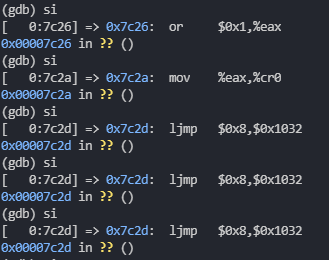
\includegraphics[width=0.8\textwidth]{cantJmp}
\quad \par 

\subsection{Exercise 6}
\textsl{Examine the 8 words of memory at 0x00100000 at the point the BIOS enters the boot loader, 
        and then again at the point the boot loader enters the kernel. Why are they different? 
        What is there at the second breakpoint?} \par 
\quad \par
在BIOS引导进入boot loader前,0x0010000处内容为空;
进入kernel前,0x0010000处已经有了内容,前后的区别在于kernel被加载进来了。

\lstset{style=AssemblyStyle}
\setmainfont{Consolas}
\begin{lstlisting}
(gdb) b *0x7c00
Breakpoint 1 at 0x7c00
(gdb) c
...  
(gdb) x/8x 0x0010000
0x10000:        0x00000000      0x00000000      0x00000000      0x00000000
0x10010:        0x00000000      0x00000000      0x00000000      0x00000000
(gdb) b *0x7d81
Breakpoint 2 at 0x7d81
(gdb) c
...
(gdb) x/8x 0x0010000
0x10000:        0x464c457f      0x00010101      0x00000000      0x00000000
0x10010:        0x00030002      0x00000001      0x0010000c      0x00000034
\end{lstlisting}
\setmainfont{Times New Roman}

\chapter[\Large The Kernel]{The Kernel}
\section[\large Using virtual memory to work around position dependence]{Using virtual memory to work around position dependence}
在前面的内容中我们已经知道,在BootLoader阶段,虚拟地址与物理地址是完全相同的(OBJDUMP对Boot的反汇编结果)。
而Kernel则不同,它会将自己映射到32-bit物理地址空间的高位:以JOS为例,它将内核映射到 0xf0100000 虚拟地址处。
由于许多PC并不具有如此大的物理内存,因此会选择将高位虚拟地址映射到低位物理地址。 \par 
JOS在启动真正的分页服务前,会使用 kern/entrypgdir.c 进行初映射,将高位/低位的4MB虚拟地址全部映射到低位4MB物理地址。

\subsection{\large Exercise 7}
\textsl{Use QEMU and GDB to trace into the JOS kernel and stop at the movl \%eax, \%cr0. 
        Examine memory at 0x00100000 and at 0xf0100000. Now, single step over that instruction 
        using the stepi GDB command. Again, examine memory at 0x00100000 and at 0xf0100000.} \par 
\quad \par
\textbf{设置CR0寄存器的PG位后,处理器进入分页模式(见IA32-3A)},运行上述命令后 entrypgdir.c 设置的分页生效。
查看 \textsl{kernel.asm} 文件得到设置 CR0 寄存器的指令(链接)地址为 0xf0100025,且此时 CPU 的分页功能
尚未生效,故实际指令地址应为 0x100025。设置断点,查看GDB前后差异,发现设置前 0xf010000 处无内容,设置后与 0x100000 
处内容相同。 \par
\quad \par
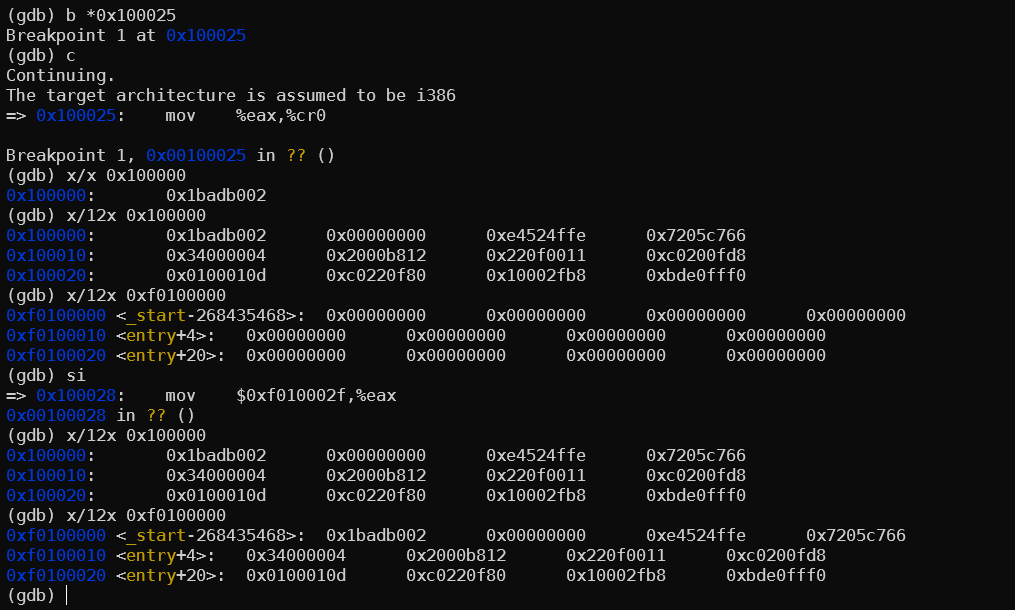
\includegraphics[width=\textwidth]{entrypgdir_start} \par

\section[\large Formatted Printing to the Console]{Formatted Printing to the Console}
这一节要求我们阅读 kern/printf.c,lib/printfmt.c 和 kern/console.c 的源码,理解它们之间的关系。\par 
分析较高调用层(如 kern/init.c)中对输出函数的使用,我们可以知道用户层的接口应该是 cprintf。
本节内容结合Question及Exercise 8来展开。\par
\textsl{注:cprintf 与 printf 的区别在于后者可以被重定向到输出屏幕之外的位置(标准输出流),前者只能输出到控制台。} \par 


\subsection{\large Question}
\textsl{1. Explain the interface between printf.c and console.c. 
        Specifically, what function does console.c export? 
        How is this function used by printf.c?} \par
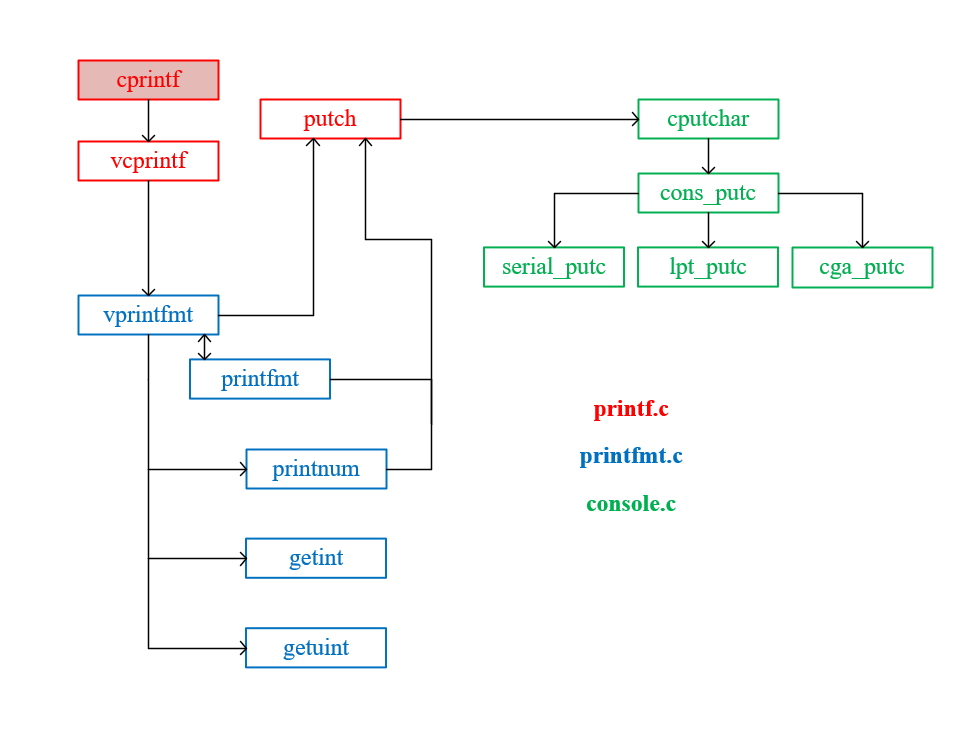
\includegraphics[width=\textwidth]{cprintf_callchain} \par
根据对三个文件的分析,我们可以大致得到调用关系如上图。
其中 printf.c 提供最外层的用户接口,并调用由 printfmt.c 及 console.c 提供的底层实现接口;
console.c 主要提供了 cputchar 函数,它调用底层接口将字符输出到控制台(屏幕)上。 \par 
\quad \par


\textsl{2. Explain the following from console.c:} \par
\lstset{style=CStyle}
\setmainfont{Consolas}
\begin{lstlisting}
if (crt_pos >= CRT_SIZE) 
{
        int i;
        memmove(crt_buf, crt_buf + CRT_COLS, (CRT_SIZE - CRT_COLS) * sizeof(uint16_t));
        for (i = CRT_SIZE - CRT_COLS; i < CRT_SIZE; i++)
                crt_buf[i] = 0x0700 | ' ';
        crt_pos -= CRT_COLS;
}
\end{lstlisting}
\setmainfont{Times New Roman} \par
这段代码出现在 cga\_putc() 函数中。CGA指的是彩色图形适配器(Color Graphics Adapter),这个函数
用于将字符串显示到CGA设备上。根据代码分析,猜测为当输出内容溢出屏幕显示范围时,将终端上第一行移出屏幕,
其他行整体上移,并将新数据写到显示器最后一行上。 \par 
\quad \par 
\quad \par

\textsl{3. Trace the execution of the following code step-by-step:} \par
\lstset{style=CStyle}
\setmainfont{Consolas}
\begin{lstlisting}
int x = 1, y = 3, z = 4;
cprintf("x %d, y %x, z %d\n", x, y, z);
\end{lstlisting}
\setmainfont{Times New Roman}
\quad \quad
\textsl{(i)In the call to cprintf(), to what does fmt point? To what does ap point?} \par 
\textsl{(ii)List (in order of execution) each call to cons\_putc, va\_arg, and vcprintf. 
        For cons\_putc, list its argument as well. For va\_arg, list what ap points to before and after the call. 
        For vcprintf list the values of its two arguments.} \par
\quad \par 
(i) cprintf中的fmt参数指向待输入的格式串;ap指向参数x,y,z构成的可变参数列表(1,3,4)。\par 
(ii) cons\_putc的参数是每次打印到控制台的字符ASCII码;每次调用va\_arg后,va\_list参数会逐渐减少至空;
     vcprintf的参数为:"x \%d, y \%x, z \%d\textbackslash n",(1,3,4)。\par
\quad \par 


\textsl{4. Run the following code.} \par
\lstset{style=CStyle}
\setmainfont{Consolas}
\begin{lstlisting}
unsigned int i = 0x00646c72;
cprintf("H%x Wo%s", 57616, &i);
\end{lstlisting}
\setmainfont{Times New Roman}
\quad \quad
\textsl{What is the output? Explain how this output 
        is arrived at in the step-by-step manner of the previous exercise.} \par 
\quad \par 
\%x是以16进制打印相应整数,DEC(57616)=HEX(110);\%s为打印字符串,而i以无符号整形存储(4字节),
且\underline{x86为小端机器},故4个字节依次为HEX(72),HEX(6c),HEX(64),HEX(00),分别对应ASCII码的r,l,d和空字符,
故最终打印结果为:HE110 Wolrd。\par 
\quad \par


\textsl{5. In the following code, what is going to be printed after 'y='? 
        (note: the answer is not a specific value.) Why does this happen?} \par
\quad \par 
y并没有指定参数,故非固定值。实际情况是,指令将从栈中取出变量3之后的一个整形长度值。\par 
\quad \par

\textsl{6. Let's say that GCC changed its calling convention so that 
        it pushed arguments on the stack in declaration order, 
        so that the last argument is pushed last. 
        How would you have to change cprintf or its interface so that 
        it would still be possible to pass it a variable number of arguments?} \par
\quad \par 
将变长数组参数与格式串参数位置进行调换即可。


\subsection{\large Exercise 8}
\textsl{We have omitted a small fragment of code - 
        the code necessary to print octal numbers using patterns of the form 
        "\%o". Find and fill in this code fragment.} \par
\quad \par 
根据前文对打印函数体系调用结构的分析得知需修改 printfmt.c/vprintfmt() 函数。
因此我们在其中加入处理八进制的分支,仿照处理十六进制的分支进行补充:
\lstset{style=CStyle}
\setmainfont{Consolas}
\begin{lstlisting}
case 'o':
        num = getuint(&ap, lflag);
        base = 8;
        goto number;
\end{lstlisting}
\setmainfont{Times New Roman}

\section[\large The Stack]{The Stack}
本节的内容主要关于C程序对x86的栈使用,并讨论了JOS的内核栈相关内容。\par 

\subsection{\large Exericse 9}
\textsl{Determine where the kernel initializes its stack, 
        and exactly where in memory its stack is located. 
        How does the kernel reserve space for its stack? 
        And at which "end" of this reserved area 
        is the stack pointer initialized to point to?} \par
\quad \par 
内核在 kern/entry.S 中的一行代码初始化了内核栈:
\lstset{style=AssemblyStyle}
\setmainfont{Consolas}
\begin{lstlisting}
# Set the stack pointer
movl	$(bootstacktop),%esp
\end{lstlisting}
\setmainfont{Times New Roman}
\$bootstacktop 变量定义在同一文件下,在切换到.data段后定义:
\lstset{style=AssemblyStyle}
\setmainfont{Consolas}
\begin{lstlisting}
.data
###################################################################
# boot stack
###################################################################
        .p2align	PGSHIFT		# force page alignment
        .globl		bootstack
bootstack:
        .space		KSTKSIZE
        .globl		bootstacktop   
bootstacktop:

\end{lstlisting}
\setmainfont{Times New Roman}
使用GDB进行断点调试,链接后地址为0xf0117000(虚拟地址);通过.space指令,
内核初始化了一个大小为 KSTKSIZE=8*PGSIZE=32KB 的区域作为栈生长空间,而栈顶位于0xf0117000,
向低位地址生长。
\quad \par 

在32-bit的x86体系中,栈一般只存储32-bit的数据——也即,栈是4字节对齐的,因此存放栈顶地址的ESP寄存器
的值应当是可被4整除的。包括 call 在内的一系列x86指令,都会默认使用ESP所指的栈(Hard-wired的)。\par 
除了ESP寄存器外,x86体系中还存在一个称为\textsl{栈帧指针(Stack Frame Pointer)}的EBP寄存器,协助对栈进行维护:
当C程序发生函数调用时,它会将当前函数的EBP寄存器值入栈,并将当前ESP值复制到EBP寄存器中。有了这一规则的补充,
我们可以利用栈对调用链进行回溯。\par 

\subsection{\large Exercise 10}
\textsl{To become familiar with the C calling conventions on the x86, 
        find the address of the test\_backtrace function in obj/kern/kernel.asm, 
        set a breakpoint there, and examine what happens each time it gets called after the kernel starts. 
        How many 32-bit words does each recursive nesting level of test\_backtrace push on the stack, 
        and what are those words?} \par
\quad \par 
这个练习的目的是帮助我们了解C程序的过程调用规则。我们设置断点对 test\_backtrace 进行跟踪。
这个函数将递归调用自己,每次被调用时,参数都将减一。根据步进调试,我们可以得到该函数调用的流程:\par
\quad
\textsl{1. call 指令将返回地址入栈(\%esp值减少4)} \par 
\quad
\textsl{2. 将 \%ebp 入栈 (\%esp值减少4,累计8字节)} \par 
\quad
\textsl{3. 将\%esp值赋给\%ebp } \par 
\quad
\textsl{4. 将\%ebx,\%esi入栈(约定保护的寄存器值)(\%esp值减少8,累计16字节)} \par 
\quad
\textsl{5. 将\%esp减去8(0x8)个字节 (累计24字节)} \par 
\quad 
\textsl{6. 将\%esi,\%eax入栈(\%esp值减少8,累计32字节)【vprintf调用参数】} \par 
\quad
\textsl{7. 调用 vprintf 后将\%esp加上16(0x10)个字节(累计16字节)【弹出参数】} \par
\quad 
\textsl{8. 递归调用自己}  \par 
\quad \par 
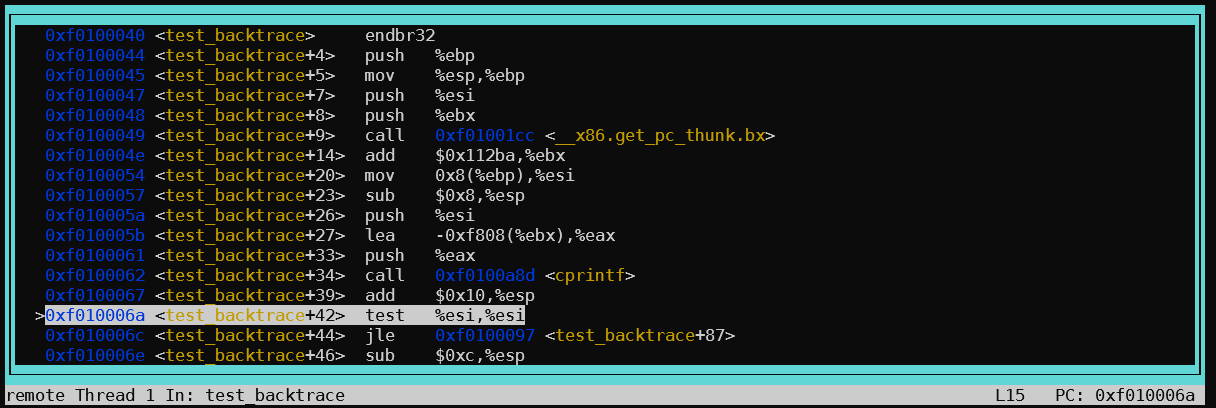
\includegraphics[width=\textwidth]{test_backtrace}
\quad \par
上面的Exercise提供了一个栈帧的实例,我们进一步分析栈在过程调用中的变化。\par 
大部分的过程使用的栈帧都是定长的:也即,在编译过程就确定并分配了定长栈帧。当发生调用时,
首先有返回地址和EBP寄存器值依次入栈,并修改EBP值;同时,它将需要保存的寄存器入栈(如上例中的EBX、ESI),并将调用
参数放入已保存的寄存器中,用于数据传送;随后为局部变量划定空间并入栈。我们知道,x86体系用于传递参数的
寄存器仅有6个,若需要更多的参数,可在栈顶继续逆序构造(第7个参数将位于低地址处)。 \par 
由于C本身支持定长数组,且C标准库中包含像alloca这样提供栈空间分配的函数,因此栈也需要支持变长特性,这一特性可以依赖
EBP实现。在早期x86代码中,每个函数都使用帧指针。如今只有栈帧长可变的情况下才使用。 \par 
\quad \par
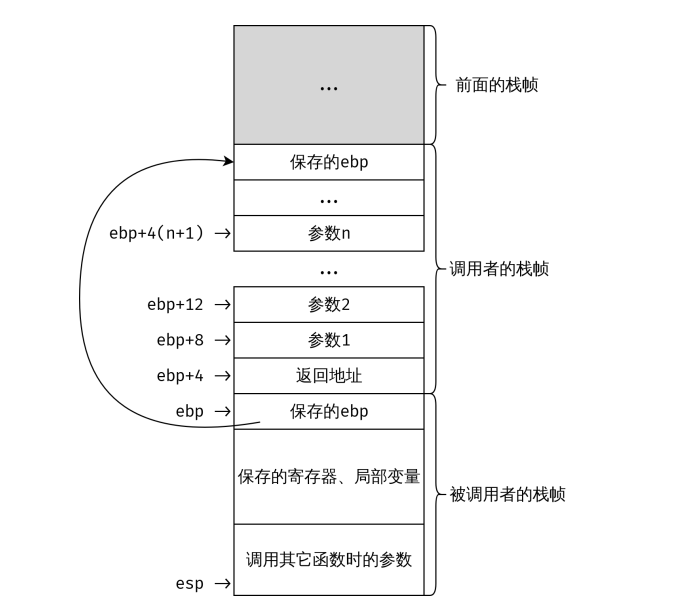
\includegraphics[width=\textwidth]{StackFrame}

\newpage
\subsection{\large Exercise 11}

\lstset{style=AssemblyStyle}
\setmainfont{Consolas}
\begin{lstlisting}
# The backtrace function should display a listing of function call frames in the following format:

Stack backtrace:
    ebp f0109e58  eip f0100a62  args 00000001 f0109e80 f0109e98 f0100ed2 00000031
    ebp f0109ed8  eip f01000d6  args 00000000 00000000 f0100058 f0109f28 00000061
...
\end{lstlisting}
\setmainfont{Times New Roman}

\textsl{Implement the backtrace function as specified above. 
        Use the same format as in the example, since otherwise the grading script will be confused.} \par
\quad \par 
这是要求我们实现backtrace功能,其原理依据正是我们上文对栈帧结构的分析。
实际需要填写的函数是 mon\_backtrace,并可以使用 read\_rbp() 接口获得EBP寄存器的值。
需要注意的是此处传递给 cprintf 的参数(指针本身的值or指针所指内存中的值):\par 
\lstset{style=CStyle}
\setmainfont{Consolas}
\begin{lstlisting}
int
mon_backtrace(int argc, char **argv, struct Trapframe *tf)
{
        // Your code here.
        cprintf("Stack backtrace:\n");

        int* now_ebp = (int *)read_ebp();
        while(now_ebp != NULL)
        // when the bootstack was initialized the 
        // ebp was also initialized with 0 and pushed
        // into the bootstack
        {
                // print ebp and eip(in *(now_ebp + 1))
                cprintf("ebp %08x eip %08x args", now_ebp, *(now_ebp + 1));
                for(int i = 1; i <= 5; ++i)
                {
                        // print the first 5 args
                        cprintf(" %08x", *(now_ebp + 1 + i));
                }
                cprintf("\n");

                now_ebp = (int *)*(now_ebp);
        }
        return 0;
}
\end{lstlisting}
\setmainfont{Times New Roman}
\quad \par 



\newpage
\subsection{\large Exercise 12}
\textsl{Modify your stack backtrace function to display, 
        for each eip, the function name, source file name, 
        and line number corresponding to that eip.} \par
\textsl{Q: In debuginfo\_eip, where do \_\_STAB\_* come from?} \par 

\quad \par 
这个Exericse要求我们利用符号表信息进一步增加backtrace的功能。根据提示,我们可以利用 
objdump 工具来查看 kernel 文件中的符号表位置(-h)与内容(-G)。其中值得注意的是符号表
段(.stab)与符号字符串表(.stabstr)段:
\quad \par
\lstset{style=MakeFileStyle}
\setmainfont{Consolas}
\begin{lstlisting}
# objdump -h obj/kern/kernel

obj/kern/kernel:     file format elf32-i386

Sections:
Idx Name          Size      VMA       LMA       File off  Algn
        0 .text         00001b9d  f0100000  00100000  00001000  2**4
                        CONTENTS, ALLOC, LOAD, READONLY, CODE
        1 .rodata       000006ec  f0101ba0  00101ba0  00002ba0  2**5
                        CONTENTS, ALLOC, LOAD, READONLY, DATA
        2 .stab         000043c9  f010228c  0010228c  0000328c  2**2
                        CONTENTS, ALLOC, LOAD, READONLY, DATA
        3 .stabstr      00001996  f0106655  00106655  00007655  2**0
                        CONTENTS, ALLOC, LOAD, READONLY, DATA
        4 .data         00009300  f0108000  00108000  00009000  2**12
                        CONTENTS, ALLOC, LOAD, DATA
        5 .got          00000008  f0111300  00111300  00012300  2**2
                        CONTENTS, ALLOC, LOAD, DATA
        6 .got.plt      0000000c  f0111308  00111308  00012308  2**2
                        CONTENTS, ALLOC, LOAD, DATA
        7 .data.rel.local 00001000  f0112000  00112000  00013000  2**12
                        CONTENTS, ALLOC, LOAD, DATA
        8 .data.rel.ro.local 00000044  f0113000  00113000  00014000  2**2
                        CONTENTS, ALLOC, LOAD, DATA
        9 .bss          00000648  f0113060  00113060  00014060  2**5
                        CONTENTS, ALLOC, LOAD, DATA
        10 .comment      0000002a  00000000  00000000  000146a8  2**0
                        CONTENTS, READONLY
\end{lstlisting}
\setmainfont{Times New Roman}
\quad \par
\newpage 
\lstset{style=MakeFileStyle}
\setmainfont{Consolas}
\begin{lstlisting}
# objdump -G obj/kern/kernel

obj/kern/kernel:     file format elf32-i386

Contents of .stab section:

Symnum n_type n_othr n_desc n_value  n_strx String

-1     HdrSym 0      1445   00001995 1
0      SO     0      0      f0100000 1      {standard input}
1      SOL    0      0      f010000c 18     kern/entry.S
...
10     SLINE  0      74     f010002f 0
11     SLINE  0      77     f0100034 0
\end{lstlisting}
\setmainfont{Times New Roman}
\quad \par
需要我们实现的代码需要利用到 kernel 中的符号表内容(.stab 段),
而符号表则通过一系列外部变量 \_\_STAB\_* 传递给程序。根据 Lab 的提示,我们在
链接脚本 kernel.ld 中找到符号表相关段落:\par 
\lstset{style=MakeFileStyle}
\setmainfont{Consolas}
\begin{lstlisting}
/* Include debugging information in kernel memory */
.stab : {
        PROVIDE(__STAB_BEGIN__ = .);
        *(.stab);
        PROVIDE(__STAB_END__ = .);
        BYTE(0)		/* Force the linker to allocate space
                                for this section */
}

.stabstr : {
        PROVIDE(__STABSTR_BEGIN__ = .);
        *(.stabstr);
        PROVIDE(__STABSTR_END__ = .);
        BYTE(0)		/* Force the linker to allocate space
                                for this section */
}
\end{lstlisting}
\setmainfont{Times New Roman}
查询链接脚本语法,我们可以对上述脚本段进行解释:
PROVIDE() 关键字相当于定义一个全局变量,外部的 C 程序可以直接引用它;
(.)英文句号为定位符号,表示当前地址,可以被赋值给变量。
由此我们可以可以知道,\_\_STAB\_BEGIN\_\_ 与 \_\_STAB\_END\_\_ 分别记录了
符号表的起始位置与终止位置。\_\_STABSTR\_BEGIN\_\_ 与 \_\_STABSTR\_END\_\_ 则
同理记录了符号字符串表的位置。 \par 
\newpage
根据上述分析,我们首先为 debuginfo\_eip 函数增添代码:
\lstset{style=CStyle}
\setmainfont{Consolas}
\begin{lstlisting}
...
// Your code here.
// lline and rline have been assigned with lline/rline in the former step
stab_binsearch(stabs, &lline, &rline, N_SLINE, addr);
if(lline > rline)
        return -1;
else
        info->eip_line = stabs[lline].n_desc;
\end{lstlisting}
\setmainfont{Times New Roman}

再修改 mon\_backtrace() 函数:
\lstset{style=CStyle}
\setmainfont{Consolas}
\begin{lstlisting}
int
mon_backtrace(int argc, char **argv, struct Trapframe *tf)
{
        // Your code here.
        cprintf("Stack backtrace:\n");
        int* now_ebp = (int *)read_ebp();
        while(now_ebp != NULL)
        {
                // print ebp and eip(in *(now_ebp + 1))
                int eip = *(now_ebp + 1);
                cprintf("ebp %08x eip %08x args", now_ebp, eip);
                for(int i = 1; i <= 5; ++i)
                        cprintf(" %08x", *(now_ebp + 1 + i));
                cprintf("\n");
                // Add EpiInfo debug information
                struct Eipdebuginfo eip_info;
                if(debuginfo_eip(eip, &eip_info) == 0)
                {
                        cprintf("\t%s:%d: %.*s+%d\n", 
                                eip_info.eip_file,
                                eip_info.eip_line,
                                eip_info.eip_fn_namelen, // see the hint in exercise12
                                eip_info.eip_fn_name,
                                eip_info.eip_fn_addr
                        );
                }
                else
                        cprintf("Error happened when reading symbol table\n");
                now_ebp = (int *)*(now_ebp);
        }
        return 0;
}
\end{lstlisting}
\setmainfont{Times New Roman}

\end{document}